\documentclass[times, 10pt,twocolumn]{article}
\usepackage{latex8}
\usepackage{times}
%\usepackage{ucs}
\usepackage{graphics}
\usepackage[utf8x]{inputenc}

%\documentstyle[times,art10,twocolumn,latex8]{article}

\pagestyle{empty}

%-------------------------------------------------------------------------
% take the % away on next line to produce the final camera-ready version
%\pagestyle{empty}
%-------------------------------------------------------------------------

\begin{document}

\title{Operating System Support for Difference-Based Partial Hardware
  Reconfiguration}

\author{Tiago de Albuquerque Reis and Antônio Augusto Fröhlich\\
  Laboratory for Software/Hardware Integration\\
  Federal University of Santa Catarina\\
  88040-900 Florianópolis -- SC -- Brazil\\
  \{reis, guto\}@lisha.ufsc.br }

\maketitle

\thispagestyle{empty}

\begin{abstract}
   Difference-based partial reconfiguration, although simpler to use by
   not needing previous floor-planning, has its utilization encouraged
   only for small changes due to its unpredictable nature. This paper
   proposes a mechanism to avoid this problem by saving the system global
   state. Therefore it doesn't matter how the difference-based partial bitstream
   will affect the hardware configuration. This way, partially reconfigurable
   system-on-chip development requires less design effort.
\end{abstract}

%-------------------------------------------------------------------------
\let\thefootnote\relax\footnotetext
{%
   This work was supported by CNPq (Conselho Nacional de Desenvolvimento Científico e Tecnológico).
}

\Section{Introduction}

% Introduce Hardware Reconfiguration as reality

Initially targeted at rapid prototyping, reconfigurable hardware
technologies such as FPGAs have found a way into quickly changing
markets during the last decade. For many electronic devices,
in-the-field upgrading becomes a must in the face of evolving
standards, particularly around multimedia and telecommunications.
Meanwhile, the scientific community has taken advantage of these
technologies to pursue the on-the-fly reconfiguration of those chips,
giving birth to a new generation of chameleon devices that can
dynamically modify their structure and behavior to match environmental
changes. Among the list of devices currently deploying this
technology, one can find multifunction personal gadgets, adaptive
switches, cognitive radios and a large number of dedicated systems.

% Make the point for software advances (hardware and tools: OK, OS:
% not OK)
 
From the hardware point of view, modern FPGAs support dynamic partial
reconfiguration, so that hardware modules can be kept in non-volatile
memory until they are required. Sophisticated
tools aid developers in tailoring designs so that logical components
can be tracked down to FPGA slices~\cite{Raghavan:2002}. From the
software point of view, however, dynamic hardware reconfiguration is
still mostly delegated to applications. Operating system support to
dynamic hardware reconfiguration is quite limited and mostly focused
on component replacement, without consistently handling side-effects
of those changes.

% Disclaimer about former Dynamic OS failures 

We are still far from a dynamic reconfiguration support system able to identify
”which”, ”when” and ”how” hardware and software components which must be reconfigured
in order to adapt a computing system to particular application demands. Indeed,
considering the dynamically reconfigurable operating systems of the 80s and 90s, like
\textsc{Apertos}~\cite{Yokote:1992} and
\textsc{Ethos}~\cite{Szyperski:1992}, whose reconfiguration
infrastructure showed very high overhead, one might conclude that the
computational cost of such infrastructure is more likely to overwhelm
the benefits associated with the technology.  Notwithstanding, the
current scenario for reconfigurable hardware brings about new
opportunities that must be investigated from a more contemporary
perspective.

% Focuses the paper: difference-based reconfiguration

In this paper, we target some major issues around
\emph{difference-based partial hardware reconfiguration}. Contrary to
module-based reconfiguration, difference-based usually requires fewer 
resources ---thus being more suitable for embedded systems--- at the
price of worsened predictability. Instead of relying on modules that have
been designed, implemented and instantiated for reconfigurability,
difference-based reconfiguration simply takes on the differences among
bitstreams, thus requiring less memory, less time and, most important,
less design effort to perform reconfigurations. Nonetheless,
foreseeing impacts on the running software in this scenario becomes
infeasible, so this kind of reconfiguration depends on the ability of
the running software to adapt itself to unstructured hardware changes.

% Reasoning about an ideal OS for difference-based reconfiguration

Within this context, we propose an operating system-level strategy to
support difference-based partial hardware reconfiguration. This
strategy is modeled around two main concepts: hardware objects that
can be dynamically created and deleted; and a mechanism to
consistently save and restore the system global state while
manipulating hardware objects. This strategy was implemented and
tested in the \textsc{Epos} System~\cite{Froehlich:2001} and will be
detailed in the next sections.

%-------------------------------------------------------------------------
\Section{Partial Hardware Reconfiguration}

%Para este trabalho, a visão de System-on-Chip adotada é a de um processador softcore sintetizado para FPGA juntamente com blocos funcionais gerenciados pelo processador e uma aplicação que executa com o suporte de um sistemas operacional. Esses blocos são utilizados pelas aplicações como coprocessadores específicos (figura \ref{fig:soc}). Como a necessidade da aplicação pode mudar com o tempo, deseja-se que esse blocos possam ser modificados ou substituídos.
In this work, our vision of system-on-chip is a softcore processor on a FPGA that may control application-specific hardware coprocessors and an application that runs with an operating system support (Figure \ref{fig:soc}). As the application's needs may change during the execution, it's desirable that these coprocessors can be modified or replaced.

%Do ponto de vista do hardware, necessita-se reconfigurá-lo para aplicar as alterações necessárias, o que ocorre a partir de uma bitstream parcial. Do ponto de vista do software, é necessário que ele se adapte à nova configuração do hardware.
Concerning the hardware, it needs to be reconfigured to apply the desired modifications, which is done by a partial bitstream. Concerning the software, it needs to adapt to the new hardware configuration.

\begin{figure}[!htb]
\centering
\resizebox{5cm}{!}{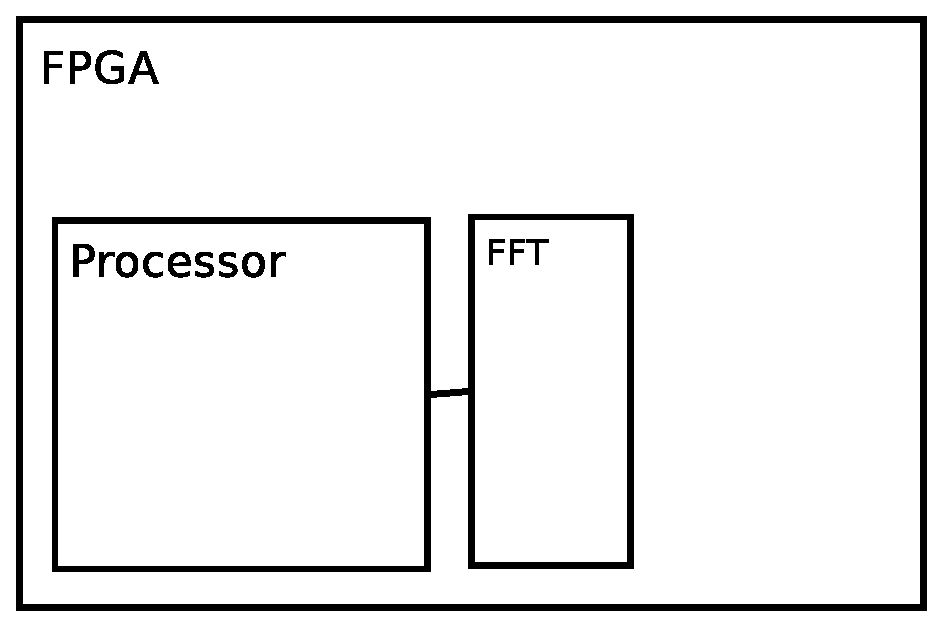
\includegraphics{figuras/soc.eps}}
\caption{System-on-Chip example}
\label{fig:soc}
\end{figure}

\SubSection{Partial Bitstreams}

%Existem duas metodologias para se obter bitstreams para reconfiguração parcial, baseada em módulos e baseada em diferenciação. A primeira atualmente é a mais utilizada em projetos de pesquisa pois provê uma estruturação modular que permite aplicar soluções análogas a sistemas computacionais convencionais. Isso ocorre pois pode-se ter na área da FPGA regiões reconfiguráveis bem definidas que facilitam a estruturação de barramentos e redes de interconexão. Baseado nessa idéia, surgiram várias arquiteturas que permitem a substituição de módulos dentro da FPGA como se fossem placas em uma placa-mãe~\cite{bobda2005esm}.
There are two methodologies for generating partial bitstreams: module-based and difference-based partial reconfiguration. The first is the most used in research projects because of its modular structuring, allowing the utilization of conventional computer system solutions. This is achieved by defining reconfigurable regions on the FPGA area that can be easily structured in buses or interconnection networks. Based on this idea, some architectures proposed the module switching and reconfigurable space organization analogous to a PC motherboard~\cite{majer2007esm}.

%Tais sistemas tem como grande vantagem a possibilidade de controlar a inserção, remoção e substituição de módulos pelo software de maneira simples, pois só é necessário indicar aonde está o bitstream parcial que os mecanismos se encarregam de incluir em algum 'slot' disponível~\cite{gonzalez2007sre,ullmann2004frt,bobda2005esm}. Apesar do ganho em simplicidade de entendimento e utilização, esses sistemas precisam de um planejamento anterior e as soluções ficam atreladas a um determinado modelo de FPGA, pois as regiões são definidas através da especificação de pontos físicos da FPGA. Além disso, uma parte considerável da área é utilizada somente pelo barramento ou rede de interconexão diminuindo a área útil para os módulos que irão realmente fazer o trabalho. Outro ponto importante é que em geral esses 'slots' tem um tamanho pré-definido que pode causar fragmentação da área útil da FPGA~\cite{steiger2004osr} ou, no pior dos casos, o módulo não caber.
Such systems have the advantage of controlling the modules' insertion, removal and substitution through software in a simple way, just by pointing to the partial bitstream's location, the mechanisms can find the appropriated module slot for reconfiguration~\cite{gonzalez2007sre,ullmann2004frt,majer2007esm}. But for this gain in the simplicity of utilization and understanding, these systems need a previous floor-planning step and the solutions tend to be focused on a FPGA model due to the reconfiguration region being physically specified on the FPGA. Besides, the bus or interconnection network share valuable design-space with the modules that actually do the work. It's also important to remember that these module slots have a pre-defined size, which may cause design-space fragmentation~\cite{steiger2004osr} or, even worse, a module may not fit.

%A segunda alternativa é pouco utilizada e tem seu uso encorajado somente para modificações pontuais como mudanças em equações de LUTs, em conteúdo de Block RAMs e em padrão de portas de entrada e saída~\cite{xilinxDSRG}. Apesar de não ser pretendida(intended) para reconfigurar grandes pedaços de lógica ela pode ser usada para esse fim. Para isso, basta se ter o design original e modificá-lo como desejado sem nenhuma restrição de local ou tamanho ou planejamento (floor-planning) prévio. A sua desvantagem nesse sentido é que aonde fisicamente essa alteração irá ocorrer não pode ser previsto. Devido a algoritmos de otimização utilizados por sintetizadores, uma pequena alteração em uma parte da lógica pode acarretar em uma grande diferença entre os designs no final.
The other way of obtaining partial bitstreams is through difference-based design, which has its use recommended for small changes like LUT equations, BlockRAM contents and I/O standards only~\cite{xilinxDSRG}. Although it is not intended to reconfigure large amounts of logic, it can still be used for this purpose. This way, it's only necessary to modify the original design to get a partial bitstream without worrying about reconfigurable regions and sizes or previous floor-planning. The disadvantage here is the unpredictability of the reconfiguration place. Because of optimization algorithms executed during the hardware synthesis, a small alteration on the logic may propagate, causing a large difference between designs.

%Para exemplificar consideremos um exemplo prático: um System-on-Chip contendo um processador softcore alojado em uma área reconfigurável que controla módulos funcionais. Com reconfiguração parcial baseada em módulos, sabe-se exatamente onde esses módulos (ou slots para eles) se encontram e qualquer modificação neles ou substituição deles pode ser controlada pelo software que executa no processador de modo 'on-the-fly' (figura \ref{fig:mbased}). Com a reconfiguração parcial baseada em diferenciação, as imprevisíveis mudanças podem ocorrer inclusive na estrutura do processador impedindo que qualquer software permaneça rodando durante a reconfiguração. Um exemplo é a configuração da FPGA da figura \ref{fig:soc} se tornar a da figura \ref{fig:dbased}, após uma reconfiguração.
Module-based partial reconfiguration lets us know exactly where slots and modules are, and its modification or substitution may be controlled on-the-fly by the software running on the processor (Figure \ref{fig:mbased}). With difference-based partial reconfiguration the unpredictable changes may happen inside the processor area, thus making it impossible to have any software running over it during the modification. An example would be Figure \ref{fig:soc}'s configuration becoming Figure \ref{fig:dbased}'s after a reconfiguration.

\begin{figure}[!htb]
\centering
\resizebox{5cm}{!}{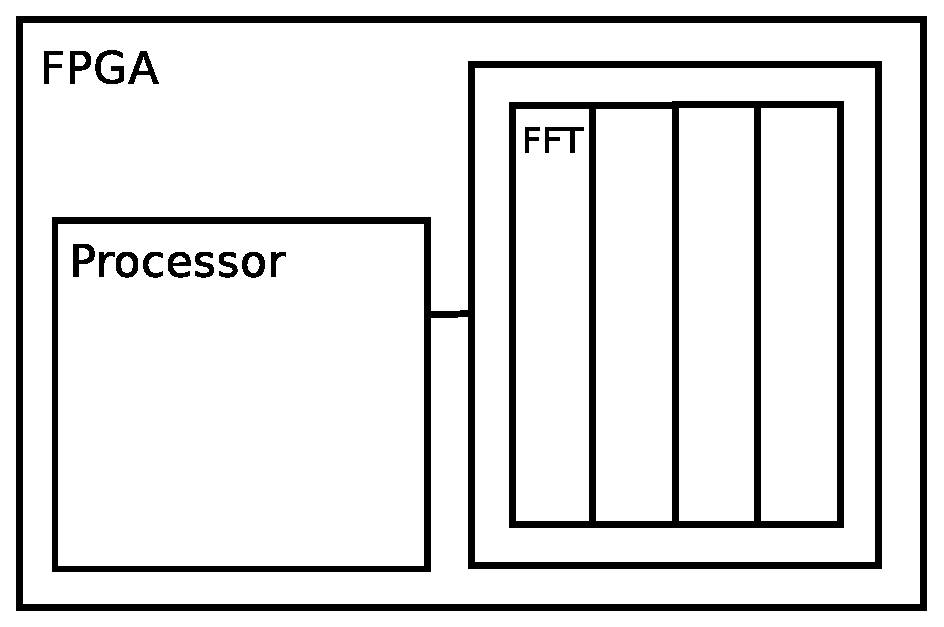
\includegraphics{figuras/mbased.eps}}
\caption{Module-based System-on-Chip}
\label{fig:mbased}
\end{figure}

\begin{figure}[!htb]
\centering
\resizebox{5cm}{!}{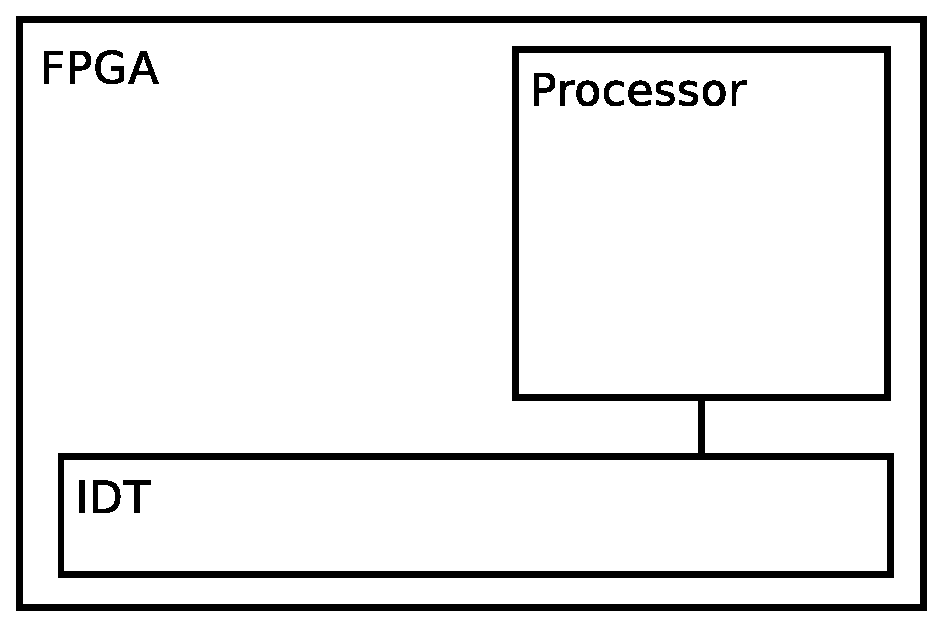
\includegraphics{figuras/dbased.eps}}
\caption{Difference-based System-on-Chip}
\label{fig:dbased}
\end{figure}


%Com um mecanismo que permita pausar a execução do software e posteriormente fazê-lo voltar a executar de onde parou, adaptando-se à nova realidade de hardware, pode-se simplificar o processo de desenvolvimento e geração de bitstreams parciais. Essa simplificação se dá pois não existe a necessidade de um planejamento (floor-planning) prévio ou de estruturação da comunicação entre CPU e módulos. Porém assim não se pode garantir que as bitstreams parciais sejam muito menores que o bitstream total, possivelmente resultando em um tempo maior de reconfiguração.
With a mechanism that allows software to pause and continue its execution and to adapt itself to the hardware's new configuration, partial bitstream development can be simplified by using difference-based bitstream generation. This simplicity comes from the lack of necessity of floor-planning or module/CPU communication structuring. Also, the design becomes FPGA-model independent and design space is saved. This may result in bigger bitstreams and consequently slower reconfiguration time because it's impossible to predict partial bitstreams sizes.


\SubSection{Software Impact}

%Uma reconfiguração no hardware pode afetar o software quando houver inserção, retirada ou modificação na estrutura de comunicação de um componente. Caso ocorra substituição de um componente tratado como um coprocessador que recebe dados e devolve resultados através de uma interface padronizada, o software não precisa adaptar-se. Como em um System-on-Chip o personagem principal é a aplicação, considera-se que cabe à ela informar ao SO como tratar o novo hardware, através de uma interface de reconfiguração de software.
A hardware reconfiguration may affect the software when a coprocessor insertion or removal happens. If it's just a modification to a coprocessor that receives data and returns results through a standardized interface, the software probably won't have to change. But this is not always the case.

As the system-on-chip's most important part is the application, it's considered that the application is responsible for informing hardware changes to the operating system, which is done through a software reconfiguration interface.

%Na inserção de um componente, o sistema operacional precisa incluir um driver que saiba onde componente está e como se comunicar com ele. Para isso, a aplicação informa através da interface o componente que deverá passar a ser suportado e o SO inicializa o driver. Considera-se que o suporte em software para o componente já esteja previamente no SO.
When a coprocessor insertion happens, the operating system needs to include a driver to communicate with it. So, using the interface, the application informs what coprocessor must now be supported and the operating system initializes the driver for it. The operating system must already have support for the coprocessor.

%Na retirada, o driver para aquele componente precisa ser excluído para evitar acessos indevidos à região onde ele se encontrava. Isso é feito informando o SO que determinado componente foi removido e a referência para ele deve ser apagada.
On the removal, excluded coprocessor drivers need to be freed from memory to avoid unwanted access to it. This is done by informing the operating system that the coprocessor was removed and references to it must be erased.

%Existe também a possibilidade de alterações na estrutura de comunicação de algum componente já conhecido, como a mudança do endereço da entrada e saída mapeada em memória do componente, que necessita de uma atualização do driver.
%There's also the possibility of changes in the communication structure of a coprocessor, like memory mapped I/O address modification, that needs a driver update.

%Assim pretende-se permitir que a aplicação tenha como fazer mudança nesses drivers, afinal esses coprocessadores em hardware estão ali à seu serviço. Mas esse suporte se dá a nível de sistema operacional para evitar que a aplicação não interfira excluindo drivers que estejam sendo utilizados por outras partes do sistema.
It is intended that the application may have a way to interfere with drivers, after all these coprocessors are there to be used by the application. This support is on operating system-level to avoid removal of drivers being used elsewhere in the system.


\SubSection{Related Work}
There are several projects aiming at enabling partial reconfiguration through frameworks or complex architectures, most of them using module-based partial reconfiguration. A simple implementation, proposed by Gonzalez~\cite{gonzalez2007sre}, defines a reconfigurable area, physically placed on a Xilinx Spartan-3 FPGA, that is connected to a MicroBlaze softcore processor. In this implementation, the reconfigurable area can be loaded with one coprocessor module, which resides on a configuration Flash memory. The execution is controlled by the application running on MicroBlaze. 

Ullmann~\cite{ullmann2004frt} proposed a more sophisticated solution for Virtex II FPGA, four reconfigurable slots are connected to each other and to the outside by a bus, which is controlled by a bus arbiter. A run-time system, running on MicroBlaze, controls the reconfiguration and is responsible for handling the incoming and outgoing messages.

Even more complex, the Erlangen Slot Machine~\cite{majer2007esm} is a complete architecture for reconfigurable computing targeting Virtex II FPGA. It's also slot-based and is concerned with very specific problems like I/O-pin dilemma, inter-module communication and local memory dilemma. It is a multi-FPGA solution, besides the main FPGA, the reconfiguration unit and a crossbar are also FPGA-based.

Such implementations are suitable for large projects with several computation units, solving problems regarding placement, communication with the rest of the system and memory access. But with little or no concern with the software part of the system. More focused on the software, Steiger et al~\cite{steiger2004osr} proposes an operating system for reconfigurable embedded systems.

This operating system is partially on software running on a general purpose CPU and partially on hardware inside a reconfigurable area. It is basically composed of a Scheduler and a Placer to manage the hardware tasks. With this functionality, a task can be placed anywhere, not limited by slots, reducing the reconfigurable area fragmentation.

Those implementations are either too simple or complex for a project that is not going to use several hardware coprocessors. Probably, a system with 2 or 3 functional units won't need a bus to communicate with the main processor, just a mapped I/O that almost doesn't impact the logic usage may be enough. Also, as the number of FPGA models increase on the market, porting the system to different models shouldn't be a complex operation. Since synthesizing tools solve all these issues, it is a clever option to let them do it.

%-------------------------------------------------------------------------
\Section{Operating System Support to Hardware Reconfiguration}

%Para permitir que o hardware seja reconfigurado sem a necessidade de reinicializar o software, é proposto um mecanismo para salvar o estado atual do software. Esse mecanismo é responsável por salvar informações relevantes para a execução do software, de modo semelhante à uma hibernação, e permitir que essas possam ser recuperadas após uma reconfiguração. Essa proposta foi implementada no sistema operacional EPOS para a arquitetura MIPS e utilizou-se o processador Plasma.
To support a hardware reconfiguration without restarting the application, this paper proposes a state saving mechanism. It is responsible for saving relevant information to the software execution for restoring afterwards, like an hibernation process. To avoid problems caused by hardware changes to the software, a software reconfiguration interface was included on the operating system, so the application can inform which drivers should be inserted to and removed from the system. The idea was implemented on the \textsc{Epos} operating system to the MIPS architecture using the Plasma softcore processor.

%parte d sw -> reconf de so

\SubSection{Background}

%EPOS é um \textit{framework} para geração de sistemas de suporte a aplicações dedicadas, permitindo o desenvolvimento de aplicações independentes de plataforma~\cite{wannerjcs2008}. Gerado após um processo de engenharia de domínio, o sistema resultante é formado somente pela aplicação e seu suporte necessário tanto em software quanto em hardware. Esse suporte vem das diversas variações e semelhanças identificadas no domínio de sistemas operacionais para sistemas embarcados: políticas de escalonamento, sincronização, temporização, gerência de memória, tratamento de interrupções e tratamento de entrada e saída~\cite{eposwso2006}.
\textsc{Epos} is a framework for building architecture independent dedicated application support systems~\cite{wannerjcs2008}. The generated system is composed only by the application and the necessary software and hardware support; this is achieved by a previous domain engineering step. The support comes from the embedded operating systems domain: scheduling politics, synchronization, timing, memory management, interrupt handling and I/O support~\cite{eposwso2006}.

%Plasma é um processador RISC softcore de 32 bits que suporta todas as instruções da arquitetura MIPS I com exceção de \textit{load} e \textit{store} desalinhadas, por serem patenteadas~\cite{plasma}. Está atualmente em sua terceira versão e é considerado estável. Por ser uma máquina MIPS, pode ser usado para executar código gerado através do compilador C da GNU, que normalmente não gera as instruções não suportadas. Possui 2 ou 3 estágios de \textit{pipeline}, controlador de interrupções, multiplicador em hardware, \textit{timer} e controladores para UART, SRAM, DDR SDRAM, Ethernet e Flash.
Plasma is a 32-bit RISC softcore processor that supports all MIPS I instructions, except the patented unaligned load and store opcodes~\cite{Plasma}. It's currently on the third version and is considered stable. The VHDL code implements either a two or three-stage pipeline, interrupt controller, hardware multiplier, timer and UART, SRAM, DDR SDRAM, Ethernet and Flash controllers.


\SubSection{System Modeling}

%Tem-se como objetivo chegar no modelo mostrado na Figura \ref{fig:sys}. Pela parte de hardware tem-se um FPGA com um processador softcore sintetizado e coprocessadores da aplicação, que podem estar atualmente no sistema ou fora dele armazenado. A qualquer momento a aplicação pode necessitar um coprocessador o que gera uma reconfiguração no hardware. No software temos o SO e uma aplicação que pode, através de uma interface, reconfigurar o software através da inserção ou remoção de drivers. Esses drivers são classes C++ inseridas no EPOS que definem como o software se comunica com o coprocessador.
Our goal is a system, like shown in Figure \ref{fig:sys}. The hardware is an FPGA with a synthesized softcore processor and application-specific coprocessors, which can be currently on the system or stored elsewhere. At any point the application may request a coprocessor, resulting in a hardware reconfiguration.

The software is an operating system with an application that can reconfigure the software through an operating system interface. This reconfiguration is done by inserting or removing coprocessor drivers, C++ classes that define how the software will communicate with the coprocessor.

\begin{figure}[!htb]
\centering
\resizebox{6cm}{!}{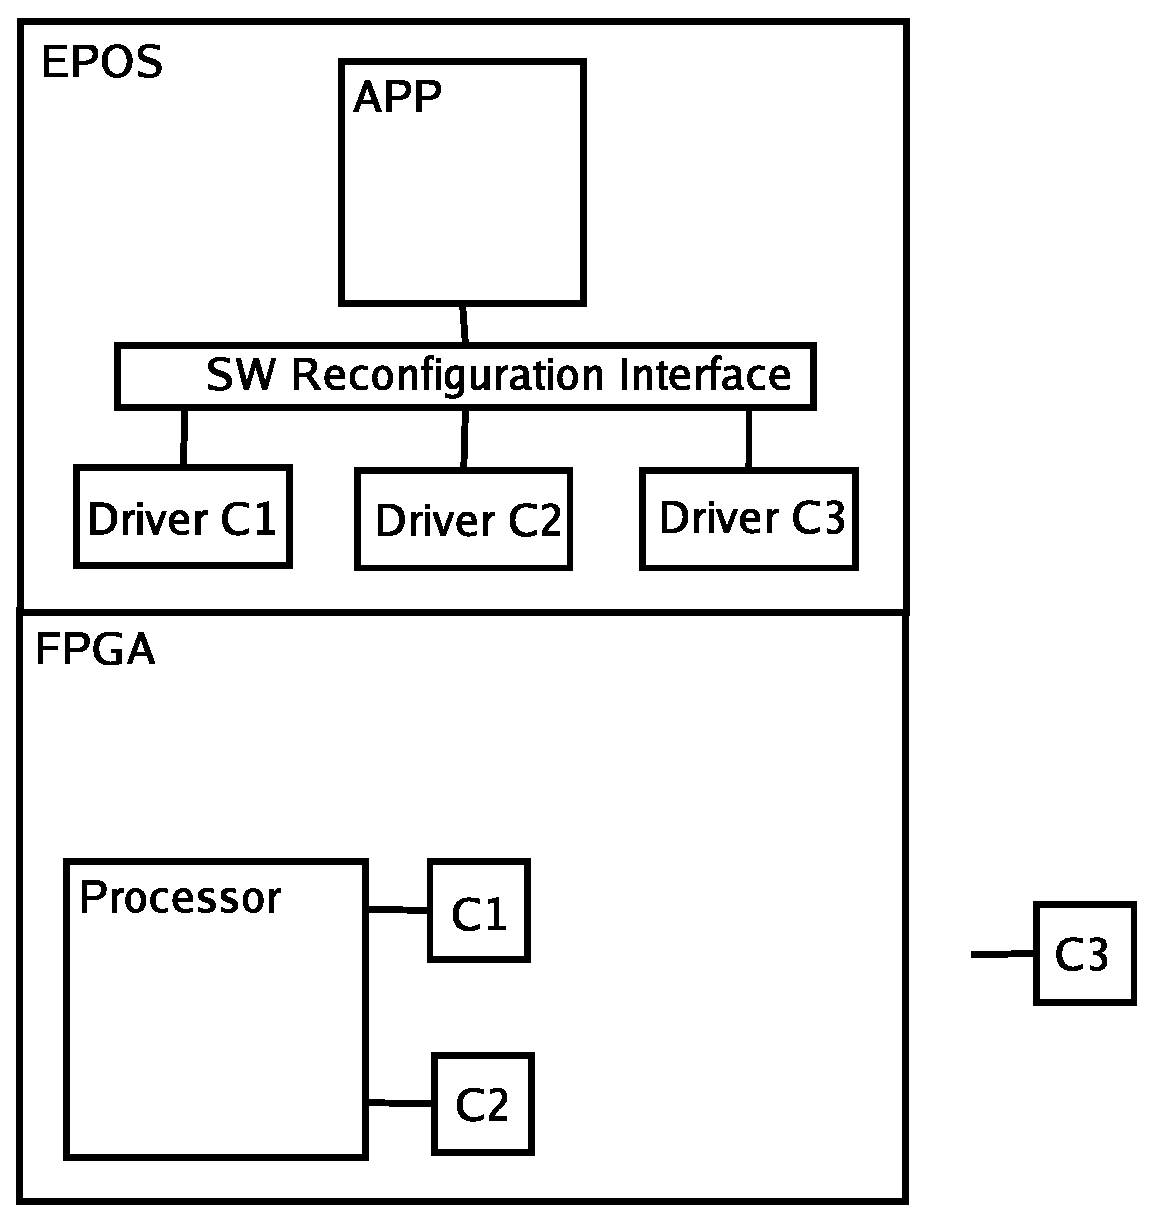
\includegraphics{figuras/sys.eps}}
\caption{The system's model}
\label{fig:sys}
\end{figure}


\SubSection{Implementation}

%Para a implementação, inicialmente foi reservado no mapa de memória do EPOS um espaço suficiente para fazer o backup dos 35 registradores da CPU e uma palavra de 32 bits para comunicação entre as execuções, como pode ser visto na figura \ref{fig:mmap}. Tomando como base a rotina assembly de salvamento de contexto da arquitetura MIPS, foi criado o método para salvar o estado do software como um todo. Além dessa rotina, modificada para salvar o contexto na região de memória reservada e sinalizar que existe um contexto a ser restaurado, também possui uma rotina opcional em C++ para fazer a cópia de todo o conteúdo da memória para uma memória não volátil. Essa rotina só é necessária para casos especiais onde se queira desligar o sistema, mas como uma reconfiguração de FPGA não necessita de um desligamento, os dados em memória RAM não são perdidos.
Initially, the \textsc{Epos} memory map was extended to accommodate 35 CPU registers and a 32-bit word for communication between executions, as seen on Figure \ref{fig:mmap}. Based on MIPS' context save assembly routine, a method was created to save the software state. Besides this assembly, modified to save the registers to a specific memory region and signalize that a context save happened, there is also a C++ routine to save the whole memory to non-volatile memory. This is executed only in cases where a system shutdown is required, since a shutdown is not needed for reconfiguration, the RAM contents are not lost.

\begin{figure}[!htb]
\centering
\resizebox{3cm}{!}{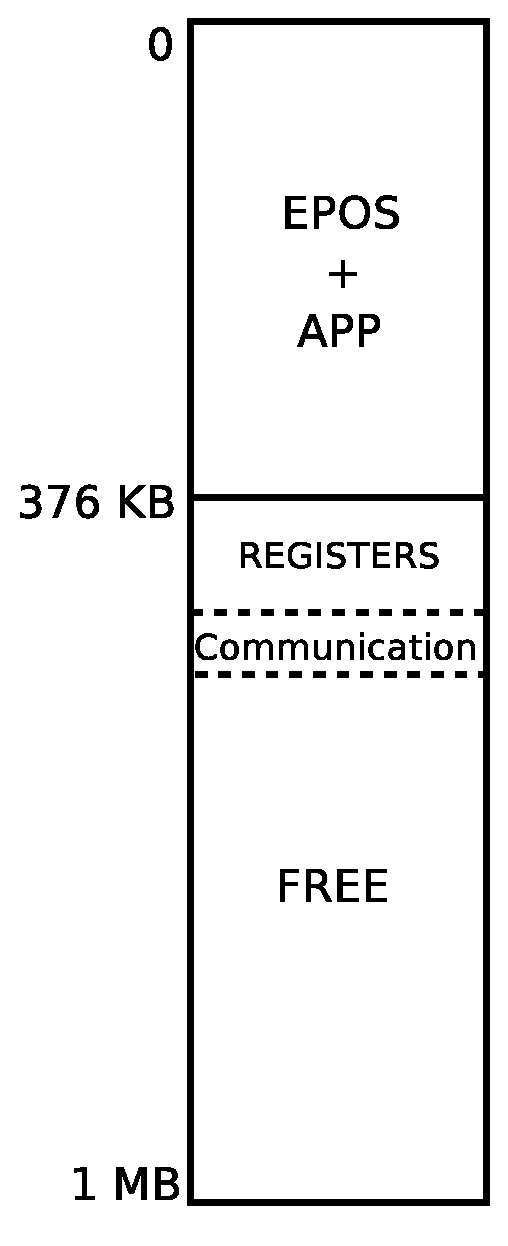
\includegraphics{figuras/mmap.eps}}
\caption{Memory Map}
\label{fig:mmap}
\end{figure}

%Antes desse método começar o salvamento, é feita uma chamada de sistema para desabilitar interrupções e assim garantir que a operação não seja interrompida. Existe também a possibilidade de se querer realizar algumas operações antes da reconfiguração mas sem que seqüelas dessa mudança permaneçam posteriormente na execução da aplicação. Para isso, após o salvamento do contexto incluiu-se uma rotina que copia todo mapa de memória do EPOS para a região de memória logo a acima dos registradores. Esses valores precisam ser recuperados futuramente logo antes da restauração do contexto da CPU pelo boot loader. 
A routine to save the memory contents to an unused part of the RAM was also included, allowing application to perform operations before the reconfiguration that will not appear in the future execution. The routine was included after the context saving. This data must be copied back before the context restore routine.

%Logo após a rotina assembly encontra-se o ponto de retorno da execução, nesse ponto precisa-se saber se o salvamento do contexto acabou de ocorrer ou se já é a nova execução. Na segunda alternativa, habilita-se o recebimento de interrupções e a execução simplesmente segue como se não tivesse parado, já na primeira é necessário salvar o conteúdo da RAM na memória não volátil ou no espaço livre da memória RAM, caso assim se queira, e parar a CPU, através do método CPU::halt(). Esse método de salvamento foi incluso no mediador do processador MIPS do EPOS e, para não interferir na pilha de execução, é um método do tipo 'inline'.
Immediately after the assembly routine is the returning point to the execution. At this point it should be known if a save or restore just happened. In the second case, the execution continues as if it had never stopped. In the first case it's necessary to copy the RAM contents to the non-volatile memory or the free space on RAM, if desired, and halt the CPU. This context saving method was included on \textsc{Epos}' MIPS processor mediator as \emph{inline}, to avoid interfering on the execution stack.

%Após a reconfiguração, o boot loader, que fica contido dentro do Plasma, é automaticamente executado e, portanto, cabe à ele decidir se o sistema está sendo iniciado pela primeira vez ou se houve uma reconfiguração e ele deve restaurar o software (figura \ref{fig:boot}). Para isso, foi adicionado um trecho de código que toma essa decisão baseado na leitura do endereço aonde o método de salvamento sinaliza. No caso da restauração, o boot loader executa uma rotina em C++ para copiar o conteúdo de uma memória não volátil ou da memória RAM para o espaço de memória do EPOS e em seguida, uma rotina assembly que recupera o contexto da CPU.
After the reconfiguration, Plasma's boot loader is automatically executed, so it has the responsibility of deciding whether the system is being turned on for the first time or a reconfiguration happened and it should restore the software (Figure \ref{fig:boot}). To achieve that, code was added to make this decision based on the content of the communication word on RAM. If a restore must happen, the boot loader executes a C++ routine to copy the non-volatile memory or RAM data to \textsc{Epos}' memory space and then an assembly routine to restore the CPU's context.

\begin{figure}[!htb]
\centering
\resizebox{7cm}{!}{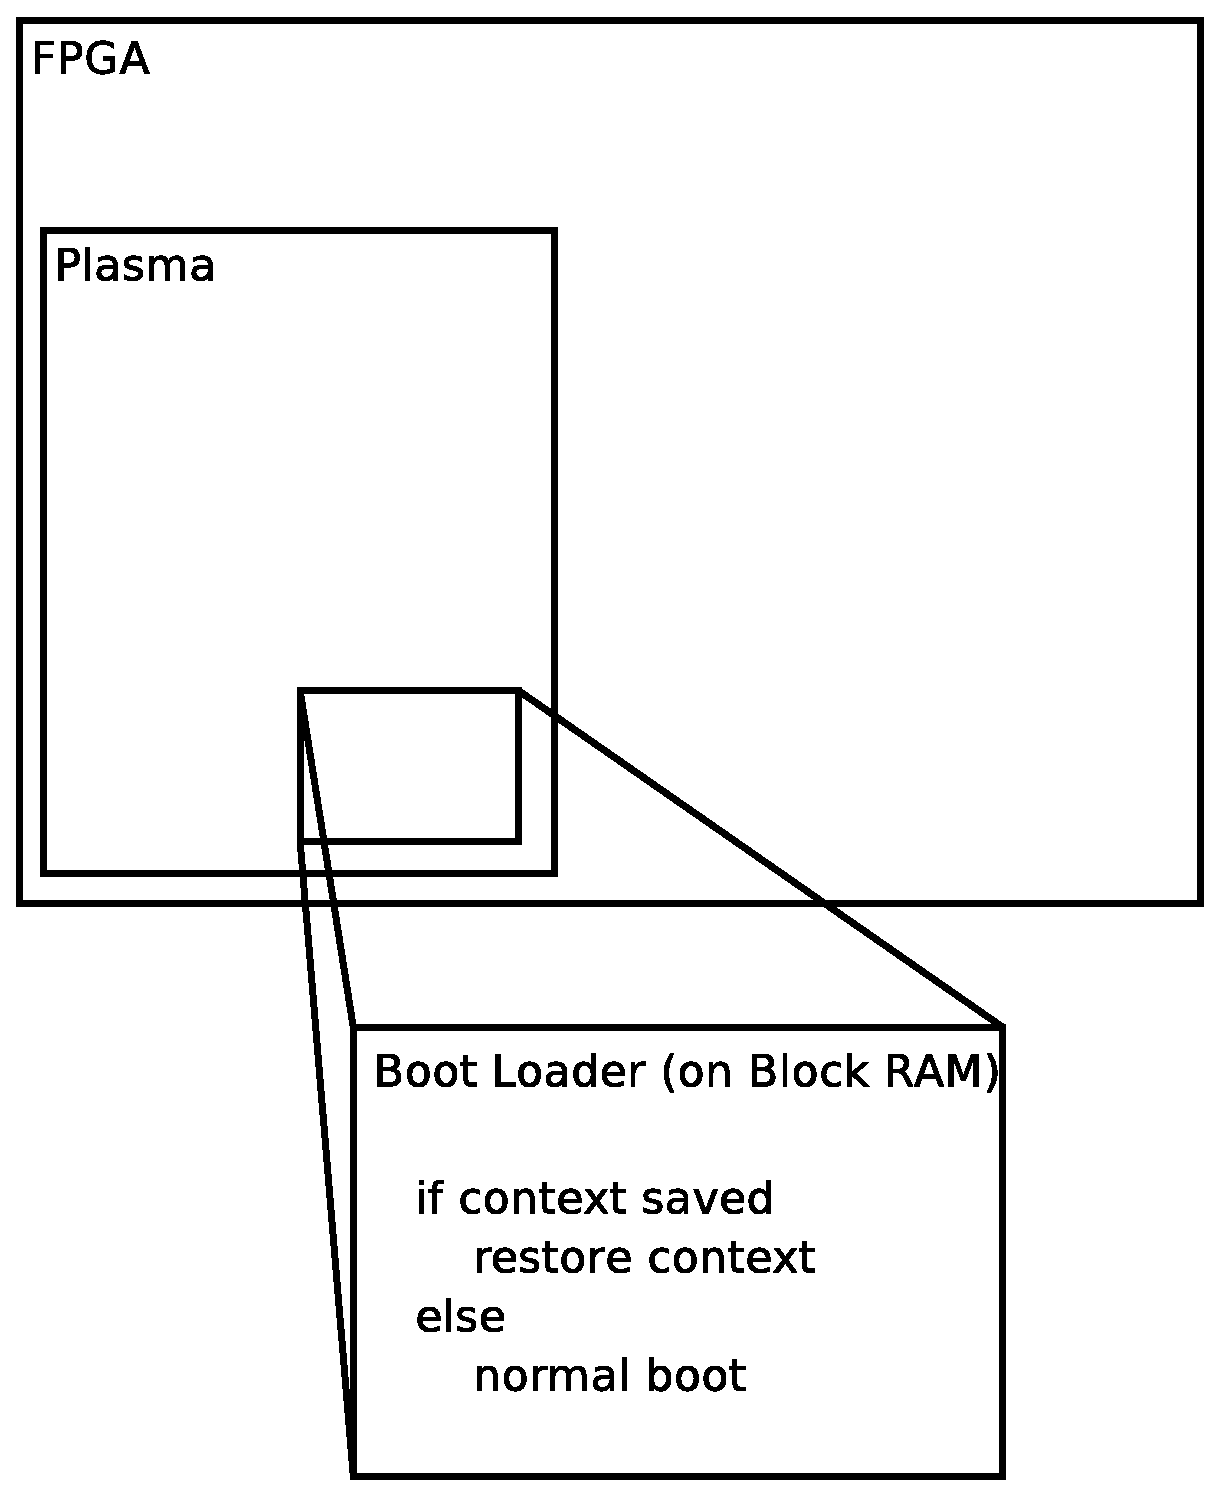
\includegraphics{figuras/boot.eps}}
\caption{Boot loader}
\label{fig:boot}
\end{figure}

%Assim que a execução retorna para a aplicação, ela deve informar ao SO quais mudanças são esperadas. Para isso, o suporte em sistema operacional provê uma API composta de dois métodos, um de inserção e outro de remoção. Para inserção, o método recebe o nome e, caso seja válido, instancia um objeto do tipo desejado. O método retorna um ponteiro para o objeto criado. Na remoção, o método recebe um ponteiro para o objeto e o apaga da memória caso não esteja sendo utilizado. Retorna um valor de estado para indicar se a remoção ocorreu ou, se não ocorreu, o porquê.
When the execution flow comes back to the application, it must inform the operating system what changes are expected. A software reconfiguration interface support was created with two methods, insert and remove. The insertion method receives the driver name and instantiates the driver object. This method returns a pointer to this object. On the removal method, the method receives a pointer to the driver's object and deletes it, returning a status code to indicate if the delete was successful and, if not, why.

\SubSection{Results and Evaluation}

%Para testar a funcionalidade do sistema foi criada uma aplicação sintética do tipo 'light-keyboard' que, logo que inicia a execução, chama o método de salvamento e pára para ser reconfigurado. Quando a reconfiguração ocorre, imediatamente os botões acendem os leds quando pressionados. Foi escolhida uma aplicação bastante simples para se ter uma melhor idéia do impacto gerado no tamanho do binário.
To test this new system functionality a \emph{light-keyboard} synthetic application that, just after starting the execution, invokes the save method and stops to be reconfigured. This reconfiguration doesn't change anything on the design, just forces Plasma to reset and execute the boot loader. After the reconfiguration, immediately the LEDs are turned on when buttons are pressed. This very simple application was used to get a better idea of the support's impact on the \textsc{Epos} binary size.

%Primeiramente mediu-se a sobrecarga desse mecanismo no tamanho do binário do EPOS. Para isso, ambas versão foram compiladas com as mesmas opções do EPOS e diretivas de compilação, assim como seus respectivos boot loaders que ficam armazenados hardcoded no Plasma. Os resultados podem ser vistos na tabela \ref{tab:binsize}. Nota-se que o código do EPOS com a aplicação aumentou 280 bytes ou 1,49\% o tamanho do sistema, enquanto que no boot loader o crescimento foi de 340 bytes ou 7,6\% mas ainda bem abaixo do limite interno do Plasma que é de 8 Kbytes.
This size overhead was measured by compiling \textsc{Epos} with and without support with the same options, the same was done to the boot loader. The results are shown on Table 1. The \textsc{Epos} binary increased 280 bytes or 1.49\% while the boot loader increased 340 bytes or 7.6\%, but still smaller than the Plasma's 8 Kilobytes internal limit.

\begin{center}
\textbf{Table 1} - \textsc{Epos} and boot loader sizes (in bytes)\\[3mm]
\begin{tabular}{|l|c|c|}
    \hline
                 & without support & with support  \\ \hline
    \textsc{Epos}& 18768  & 19048 \\ 
    Boot loader  & 4468   & 4808     \\ \hline
    \end{tabular} \\[8mm]
\end{center}

%\begin{table}[htbp]
%\begin{center}
%\caption{EPOS and boot loader sizes}
%\begin{tabular}{|l|c|c|}
%    \hline
%                 & without support & with support  \\ \hline
%    \textsc{Epos}         & 18768 Bytes & 19048 Bytes \\ 
%    Boot loader  & 4468 Bytes  & 4808 Bytes    \\ \hline
%    \end{tabular} \\[2mm]
%\label{tab:binsize}
%\end{center}
%\end{table}

%A seguir, foi medido o tempo gasto pelo mecanismo para salvar e recuperar a execução com o Plasma rodando à 25MHz. Primeiramente foi medido com a opção de salvar somente o contexto da CPU e em seguida com a cópia para memória RAM. Os resultados podem ser observados na tabela \ref{tab:tempo}. Para a medição da recuperação, a segunda tomada de tempo foi feita como primeira operação no retorno da execução. Em média, as operações com memória aumentaram o tempo de execução em 30,3 milissegundos. O salvamento em memória não volátil não pôde ser medido pela inexistência de tal tecnologia no dispositivo utilizado.
The time spent by the save and restore routines on Plasma with 25 MHz clock was also measured. The results are shown on Table 2. To measure the restore time, the second timestamp was read as the first operation after the execution flow returned to the application. The copy of RAM contents increased the operation time 30.3 milliseconds on average. The non-volatile memory copy time wasn't measured because there's no such memory on the used device.

\begin{center}
\textbf{Table 2} - Save and restore execution time (in $\mu$s)\\[3mm]
\begin{tabular}{|l|c|c|} 
    \hline
             & CPU registers only    & RAM copying \\ \hline
    Save     & 3.36      & 32203.4  \\ 
    Restore  & 26955     & 55304     \\ \hline
    Total    & 26958.36  & 87507.4  \\ \hline
    \end{tabular} \\[8mm]
\end{center}

%\begin{table}[htbp]
%\begin{center}
%\caption{Save and restore execution time} 
%\begin{tabular}{|l|c|c|} \\[1mm]
%    \hline
%             & CPU registers only    & RAM copying \\ \hline
%    Save     & 3.36 $\mu$s     & 32203.4 $\mu$s \\ 
%    Restore  & 26955 $\mu$s    & 55304   $\mu$s  \\ \hline
%    Total    & 26958.36 $\mu$s & 87507.4 $\mu$s \\ \hline
%    \end{tabular} \\[2mm]
%\label{tab:tempo}
%\end{center}
%\end{table}

%Para se testar a reconfiguração de hardware, foi desenvolvido um módulo funcional acoplado ao Plasma que tem sua execução controlada via software. Esse módulo calcula a FFT de números já contidos na memória, a partir de um dado endereço e começa sua execução à comando da aplicação.
To test the hardware reconfiguration, a FFT coprocessor was added to Plasma. This coprocessor executes a FFT algorithm over data already on memory in a given address, controlled by the application.

%A aplicação a partir do momento que faz uma chamada para inclusão do driver do módulo FFT, passa a poder controlá-lo através de chamadas de alto nível como fft\_start(), fft\_getresults() mascarando informações como endereço da memória aonde os dados são gravados e sinalização para começar ou parar a execução.
After the application tells \textsc{Epos} that a FFT coprocessor driver should be inserted, it's able control it using high level calls like fft.start() or fft.getresults(). Information like the memory address with data and signaling are masked by the driver.

%O tamanho do bitstream parcial para modificar o design atual, gerado através da diferença entre os designs foi de 123 bytes. O tempo gasto para reconfigurar não pode ser medido pois a reconfiguração é feita diretamente entre uma memória Flash de configuração e o FPGA durante a inicialização do sistema ou controlado via botão presente na placa. Esse tempo pode ser estimado tomando como base a velocidade de comunicação entre os dois dispositivos que nesse caso é de 33 Mbits/s.
The size of the difference-based partial bitstream generated was 123 bytes. Its reconfiguration time couldn't be measured because it's done directly between the FPGA and a special configuration Flash memory. This configuration happens when the system is turned on or by pressing a button on the board. This time may be estimated based on the communication speed between the two devices: 33 Mbits/s.

Currently, a video encoder proposed by Husemann~\cite{husemann} is being integrated to Plasma to perform H.264 CIF resolution encoding at 30 frames per second. In his work, Husemann presented an approach to increase the performance of Motion Estimation (ME) algorithm by using two complementary techniques, 4:1 sub-sampling and truncation of two least significant bits of each sample. This gain of performance results in a small quality loss (lower than 0.25 dB). Although small, this noise can be a problem if the original image sequence has low temporal redudancy. So this ME algorithm will only be used to encode sequences that produce acceptabe noise, being reconfigured to a standard algorithm if a low temporal redundancy image sequence is detected.



%-------------------------------------------------------------------------
\Section{Conclusion}

%Este trabalho propôs que é viável a utilização de reconfiguração parcial baseada em diferenciação para modificação de System-on-Chips, driblando sua imprevisibilidade na geração de bitstreams parciais. Isso é feito através de um mecanismo de salvamente e recuperação de contexto de execução.
This paper proposed that difference-based partial reconfiguration is viable for system-on-chip development if its bitstream generation unpredictability can be avoided. This is done by a software state save and restore mechanism.

%Como mudanças no hardware causam impacto no software, este trabalho também propôs uma interface entre a aplicação e o sistema operacional para que ela possa informar que coprocesadores saíram ou entraram no sistema. Essa tarefa é considerada da aplicação pois, além de utilizar, é ela que solicita as mudanças no hardware.
As hardware changes impacts the software running over it, this work also proposes a software reconfiguration interface to allow the application to inform the operating system about the coprocessors entering and leaving the system. This is considered an application job because it is the application which requests coprocessor changes, besides using them directly.

%Assim pode-se ter um System-on-Chip parcialmente reconfigurável sem a necessidade de estruturação do FPGA através de barramentos ou redes de interconexão.
This way, a partially reconfigurable system-on-chip can be designed without intermodule communication structuring such as buses or interconnection networks on the FPGA, simplifying the design, saving design space and making it model-independent.

%-------------------------------------------------------------------------

\bibliographystyle{latex8}
\bibliography{latex8}
\end{document}
